\section{Experiments}
\label{sec:experiments}
In this section, we evaluate the effectiveness of \method\ in terms of \textit{accuracy} and \textit{efficiency}, both of which are important in practical data valuation systems. Specifically, we first perform two types of counterfactual evaluations to quantitatively study data valuation accuracy of \method\ on small-scale setups (Section~\ref{sec:brittleness}). Then, we scale \method\ to LLMs and their massive training data, where we investigate qualitative accuracy (\ie,\ how similar most valuable training data are to the model output) and memory/compute efficiency (Section~\ref{sec:llm}). Finally, our appendix includes more qualitative results of data valuation (Appendix~\ref{sec:qualitative}), pseudo-code for LLM experiments (Appendix~\ref{sec:code}), and experimental details such as hyperperameters and compute resources (Appendix~\ref{sec:hyperparams}).


\subsection{Quantitative Accuracy with Counterfactual Evaluation}
\label{sec:brittleness}

\begin{figure}[htbp]
    \centering
    \begin{subfigure}[b]{\textwidth}
        \centering
        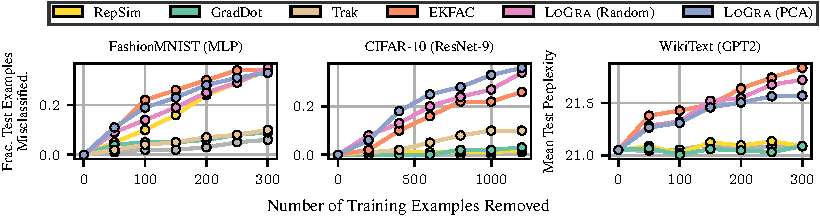
\includegraphics[width=0.97\textwidth]{figures/logra_subset_removal.pdf}
        \vskip -3pt
        \caption{Brittleness test}
        \label{fig:subset}
    \end{subfigure}
    \vskip 5pt
    \begin{subfigure}[b]{\textwidth}
        \centering
        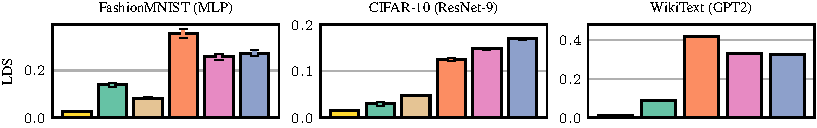
\includegraphics[width=0.97\textwidth]
        {figures/logra_lds_bar.pdf}
        \vskip -3pt
        \caption{Linear datamodeling score (LDS)}
        \label{fig:lds}
    \end{subfigure}
    \vskip -3pt
    \caption{Quantitative accuracy evaluation of data valuation algorithms. We excluded TRAK in the WikiText experiments due to lack of a public implementation for language modeling tasks.}
    \label{fig:quantitative}
\end{figure}

To quantitatively assess accuracy of data valuation algorithms, we adopt two counterfactual evaluation methods: brittleness test~\cite{ilyas2022datamodels} and linear datamodeling score (LDS)~\cite{park2023trak}. First, the brittleness test focuses on accuracy in successfully identifying \textit{top} valuable data. To this end, it first removes the top-$k$ valuable data identified by each algorithm, retrains the model without them multiple times with different random seeds, and measures the overall change in the model output. The larger the output change is, the more accurate the algorithm is in identifying \textit{top} valuable data. Second, LDS measures general valuation accuracy of \textit{all} training data under the additivity assumption. Specifically, given multiple data subsets $\{S_i\}$ of the fixed size (\eg,\ $|S_i|=|D|/2$), LDS estimates the test performance of the model trained on $S_i$ by summing the values of all examples in $S_i$ returned by each algorithm, and compares it against the gold performance obtained by actually training the model on $S_i$ using the Spearman correlation. Noting that linear datamodels have a connection to the game-theoretic data value (\eg,\ Shapley value)~\cite{ilyas2022datamodels}, LDS can serve as a principled way to study data valuation accuracy.

We perform these counterfactual evaluations on three benchmarks where many rounds (up to 1800) of retraining is feasible: (1) MLP with FMNIST, (2) ResNet-9~\cite{he2016deep} with CIFAR-10, and (3) GPT2~\cite{radford2019language} with WikiText. On these benchmarks, we compare accuracy of \method\ against four popular data valuation baselines, including gradient dot product~\cite{pruthi2020estimating}, TRAK~\cite{park2023trak}, EKFAC influence~\cite{grosse2023studying}, and representation similarity~\cite{hanawa2020evaluation}. With the aim of bearing relevance to a large-scale setting with LLMs and their vast training data, we have only considered baseline methods that satisfy the following two conditions. First, the method cannot retrain the model multiple times for identifying top-$k$ valuable data.\footnote{Note that multiple retraining is only allowed for evaluating accuracy of already identified top-$k$ data, but not for identifying top-$k$ data itself in our experiments.} Second, the method only has access to the final model checkpoint, which is the case for most LLMs. Given the above setup, we present our experiment results in Figure~\ref{fig:quantitative}.

We observe that \method\ slightly underperforms EKFAC influence, which is a few orders of magnitude slower in our large-scale experiments (Section~\ref{sec:llm}), while noticeably outperforming other baselines. We attribute competitive accuracy of \method\ to two factors. First, unlike TRAK of which projection dimension is limited by the huge projection matrix, \method\ can efficiently afford a higher projection dimension thanks to its sublinear memory/compute costs for gradient projection, and thus achieve the higher expressivity.
Second, gradient projection enables \method\ to compute raw projected Fisher information matrix (or Hessian) without an approximation as in EKFAC influence. We expect that a more accurate computation of the Hessian generally leads to more accurate data valuation results.

Comparing the initialization schemes for \method\ (PCA vs. random), we observe that \method-PCA outperforms \method-random on the FMNIST and CIFAR benchmarks. Hence, we hypothesize that it is generally more accurate to compute influence functions with larger components, similar to the spectral gradient sparsification effect of a damping term we discussed in Section~\ref{sec:theory}. To understand a relatively poor performance of \method-PCA on WikiText+GPT2, we point out that the Transformer architecture~\cite{vaswani2017attention} used in this benchmark lacks the specialized KFAC Hessian approximation, unlike naive MLP~\cite{martens2015optimizing} or convolutional~\cite{grosse2016kronecker} architectures in other benchmarks. Subsequently, our ad-hoc implementation of the PCA initialization based on the naive MLP architecture (\ie,\ no weight sharing) may not successfully keep larger components of the GPT2 Hessian, failing to deliver its benefit. As a result, we decide to use \method-random for our LLM experiments in the next subsection.

\subsection{Scaling to Billion-Scale Models \& Datasets}
\label{sec:llm}
Given competitive accuracy of \method, we now evaluate its practical utility in valuing billion-scale training data for billion-scale models. Specifically, we adopt GPT2-XL (1.5B) \cite{radford2019language}, Pythia-1.4B~\cite{biderman2023pythia}, and Llama3-8B-Instruct~\cite{llama3modelcard} as our models, and conduct data valuation on a random 1B-token subset of the OpenWebText (OWT) dataset~\cite{gokaslan2019openwebtext}. The major motivations behind choosing OWT as our data valuation dataset are twofold. First, we observe that OWT consists of relatively higher-quality data compared to other LLM training datasets like C4~\cite{raffel2020exploring} or Dolma~\cite{soldaini2024dolma} while maintaining the diversity unlike other high-quality datasets like WikiText~\cite{merity2016pointer}. Second, we anticipate that OWT largely overlaps with training datasets of all our models. In detail, GPT2-XL is trained on the WebText dataset that shares the same data curation process with OWT, Pythia-1.4B is trained on the Pile dataset~\cite{gao2020pile} that includes an extension of OWT (\ie,\ OpenWebText2), and we suppose a majority of OWT would be a part of Llama3's massive 15T-token pretraining dataset. We also note that our OWT subset size (\ie,\ 1B tokens) was mainly limited by the available storage, not by compute (see Table~\ref{tab:llm_efficiency}). If we had access to a storage size of 1PB, performing data valuation with a dataset size of 100B+ tokens would be readily feasible using the same compute resource.

\textbf{Efficiency.\hspace{2.5mm}} To begin with, we compare memory and compute efficiency of \method\ against EKFAC influence~\cite{grosse2023studying}, the state-of-the-art and only algorithm that can run on billion-scale models without CUDA out-of-memory (OOM) errors. Indeed, we confirm that running TRAK or Arnoldi IF with billion-scale models results in CUDA OOM errors even on A100 GPUs with 80GB VRAM due to their gigantic projection matrix sizes. We report GPU memory usage and throughput of both logging (one-time) and influence computation (recurring) phases for the Llama3-8B-Instruct experiment with one A100 GPU and half-precision in Table~\ref{tab:llm_efficiency}.
\vskip -5pt
\begin{table}[htbp]
\centering
\scriptsize
\begin{tabularx}{\textwidth}{X*{8}{c}}
\toprule
       & \multicolumn{4}{c}{\textbf{Logging} (Compute \& save Hessian$\,$|$\,$grad)} & \multicolumn{4}{c}{\textbf{Compute Influence} (Dot product between test \& train grads)}  \\\cmidrule(r{4pt}){2-5} \cmidrule(l){6-9}
       & $\;$Batch$\;$ & $\;$Throughput$\;$     & $\;$Memory$\;$   & $\;$Storage$\;$ & $\;$Train Batch$\;$ & $\;$Test Batch$\;$ & $\;$Throughput$\;$  & $\;$Memory$\;$\\\midrule
EKFAC &1 & 1740 / 419$^*$          & 71 / 80$^*$GB & \textbf{89 GB}     & 4           & 4          & 12.2      & 75 GB  \\[0.1ex]
\method &1 & 3430 & \textbf{23 GB}   & 3.5 TB   & 256           & 4          & 1599.6      & \textbf{14 GB}  \\[0.1ex]
\method &16 & \textbf{4696} & 79 GB  & 3.5 TB    & 256           & 256          & \textbf{79003.9}      & \textbf{15 GB} \\\bottomrule
\end{tabularx}
\vskip 3pt
\caption{Memory \& compute efficiency analyses for \method\ and EKFAC. Throughput is measured as tokens/s for logging and (train, test) pairs/s for influence computations. $^*$ EKFAC logging consists of two subphases of KFAC fitting (left of /) and corrected eigenvalue fitting (right of /).}
\label{tab:llm_efficiency}
\end{table}

%EKFAC works with a raw gradient of which size is 16GB in half-precision with an 8B model, making storing raw gradients for \textit{all} training data to disk infeasible.
Due to the huge size of raw gradients (\eg,\ 16GB in fp16 for an 8B model), EKFAC cannot afford storing raw gradients for \textit{all} training data to disk.
As a result, EKFAC needs to recompute all training gradients for each test batch, and thus requires allocating extra GPU memory on model weights and intermediate activations. This largely limits both train/test batch sizes and throughput (12.2 pairs/s), and performing data valuation with EKFAC for 256 test data and 1B-token training data would take 11,300 A100 GPU hours, rendering it hardly usable in most practical setups.

In contrast, with its (efficient) gradient projection, \method\ not only significantly improves compute and memory efficiency, but also avoids training gradient recomputations at the costs of disk space for storing \textit{projected} training gradients and latency from data IO. Since the storage cost is typically much cheaper than the compute cost\footnote{\eg,\ hourly rates for a 1TB storage and one A100 GPU are approximately \$0.03 and \$4 on AWS.}, we believe our trade-off offers considerable practical benefits. Furthermore, we can largely hide the data IO cost by overlapping gradient reading/writing processes with other computations. For instance, given the fixed train gradient batch size of 256 (\ie,\ fixed data loading time), we are able to successfully overlap the process of loading training gradients from disk with influence computations against up to 256 test gradients, and thereby achieve almost 6,500$\times$ improvement in throughput from EKFAC influence. Noting that our GPU memory usage is far from saturated even with the train/test batch size of 256, we believe that more throughput improvements can be achieved simply by further increasing train/test batch sizes.
%Finally, we expect that the use of more advanced techniques like vector database~\cite{johnson2019billion} can improve efficiency by a large margin. 


\textbf{Qualitative Accuracy.\hspace{2.5mm}} Next, we analyze qualitative similarities between queried LLM outputs and most valuable data identified by \method\ that can be critical for promoting trust in the data valuation system~\cite{worledge2023unifying}. Importantly, we observe that naive influence functions frequently return outlier data with high gradient norms as most valuable data, as also noted in \cite{barshan2020relatif,grosse2023studying}. To mitigate this issue, we instead use $l$-RelatIF, a variant of influence functions that normalizes the original influence score with the self-influence score of each training data to penalize such outlier effects~\cite{barshan2020relatif}. Our experimental results are provided in Figure~\ref{fig:llm} (concise) and in Appendix~\ref{sec:qualitative} (extensive).

\begin{figure}
    \centering
    \begin{subfigure}[b]{\textwidth}
        \centering
        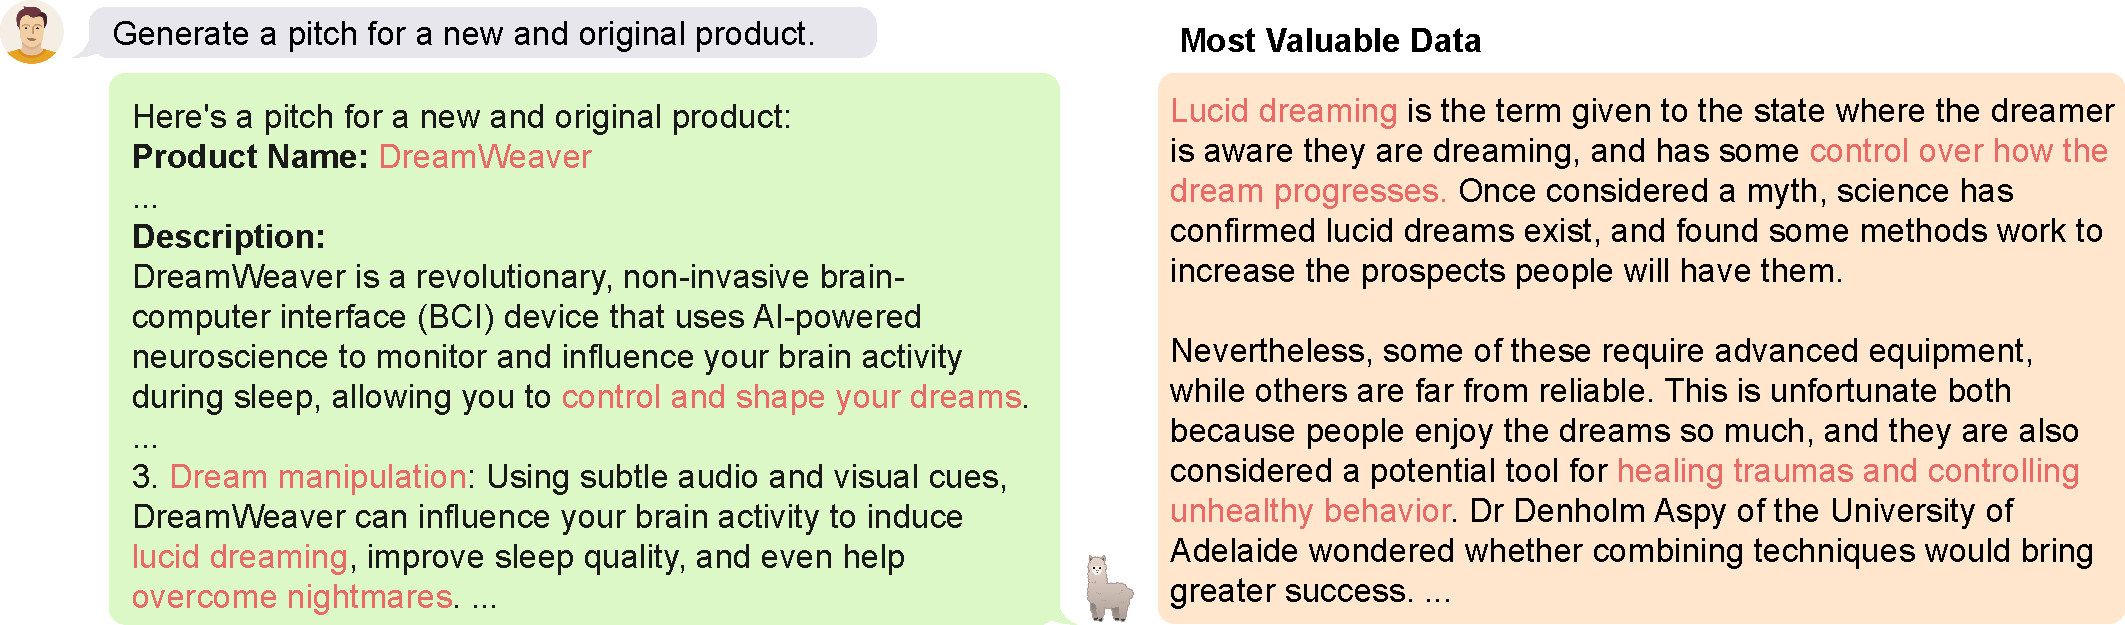
\includegraphics[width=0.98\textwidth]{figures/llama.pdf}
        \vskip -3pt
        \caption{Llama3-8B-Instruct}
        \label{fig:llama3}
    \end{subfigure}

    \begin{subfigure}[b]{\textwidth}
        \centering
        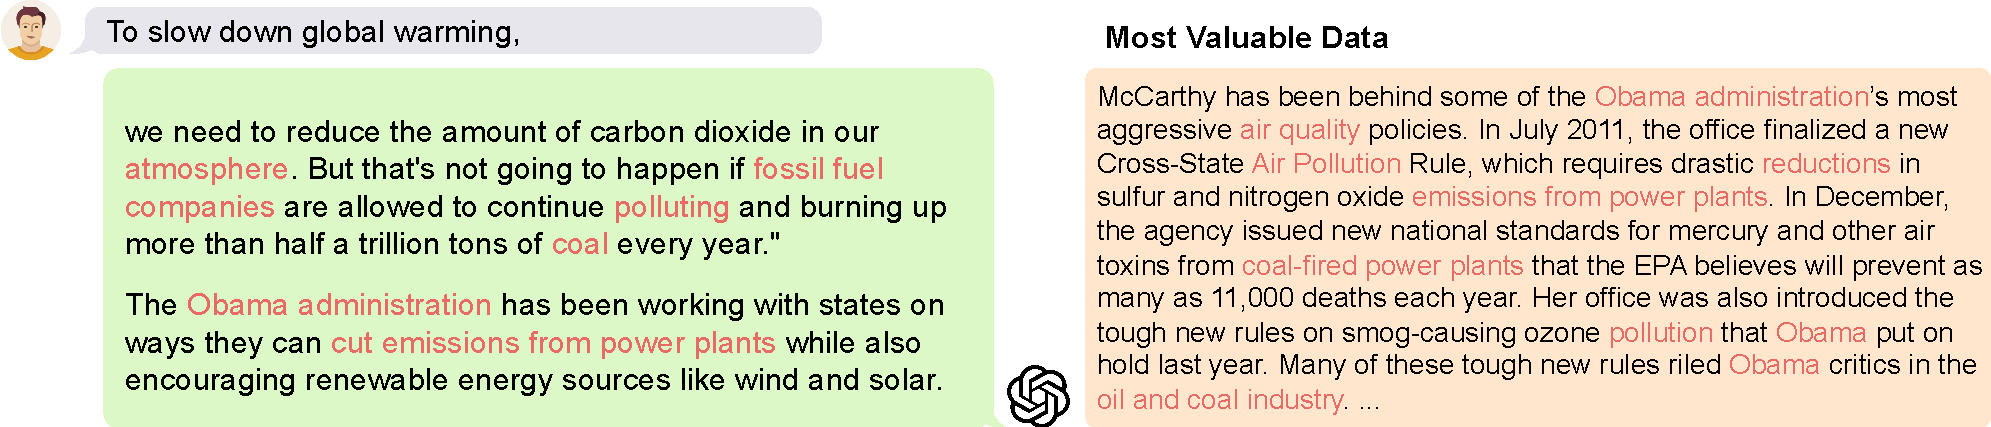
\includegraphics[width=0.98\textwidth]{figures/gpt2-main.pdf}
        \vskip -3pt
        \caption{GPT2-XL (1.5B)}
        \label{fig:gpt2}
    \end{subfigure}

    \begin{subfigure}[b]{\textwidth}
        \centering
        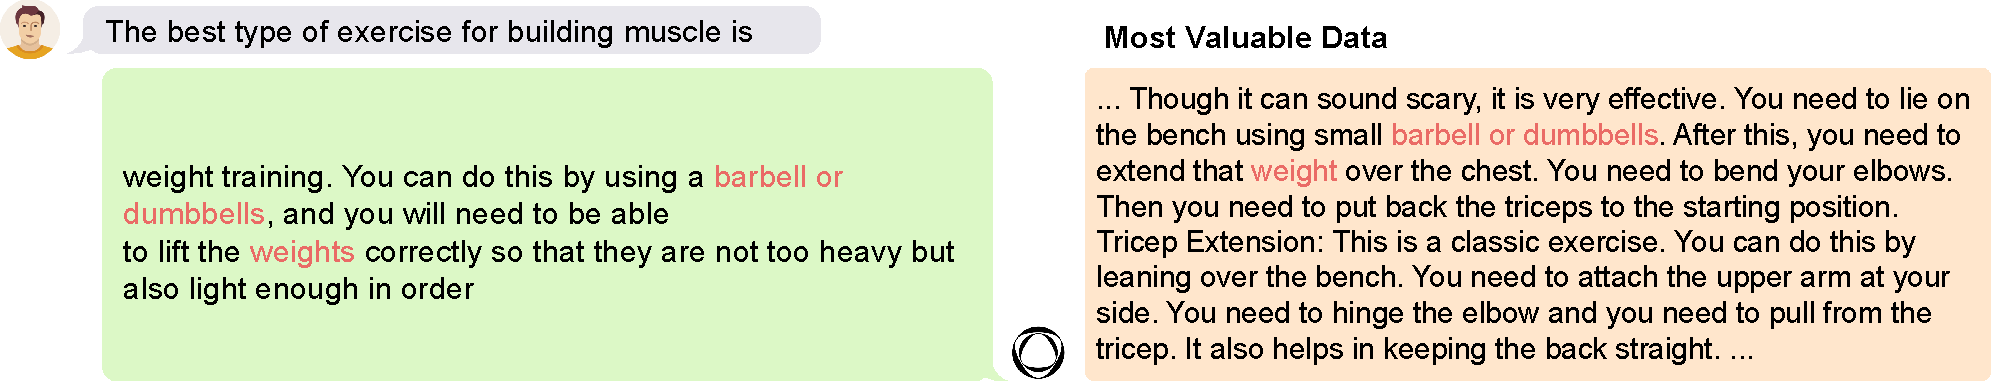
\includegraphics[width=0.98\textwidth]{figures/pythia-main.pdf}
        \vskip -3pt
        \caption{Pythia-1.4B}
        \label{fig:pythia}
    \end{subfigure}

    \caption{Qualitative accuracy of data valuations with \method. Important keywords in each example are \textit{manually} highlighted for the improved readability. More examples can be found in Appendix~\ref{sec:qualitative}.}
    \label{fig:llm}
\end{figure}

We observe that most valuable data identified by \method, especially for Llama3-8B-Instruct and GPT2-XL, share qualitative similarities (\eg,\ semantics, style, token overlaps) with the queried LLM outputs. For instance, given Llama3's response on the dream manipulation product, \method\ identifies a scientific article that studies manually inducing the lucid dream as most valuable data in Figure~\ref{fig:llama3}. In Figure~\ref{fig:gpt2}, both the GPT2-XL output and the corresponding most valuable data discuss the need for reducing emissions in the coal industry and its connection to the specific administration. In Figure~\ref{fig:pythia}, the concept of ``lifting barbell or dumbells'' appear in the model output and the most valuable data. 

However, we also notice several failure cases where the identified most valuable data seemingly do not share qualitative similarities with the LLM output, especially with Pythia-1.4B (Appendix~\ref{sec:pythia_appendix}). We here provide three potential explanations on these failing examples based on our experiments. First, attributed data may lack qualitative similarities when the queried LLM output itself is incoherent that its gradient does not encode meaningful information. This aligns with our observation that the failure case occurs more frequently with lower-tier models like Pythia-1.4B whose outputs generally are of lower quality. Second, since we only used a 1B-token subset for data valuation, it is possible that our valuation dataset may lack similar data to some queries. As noted above, our experiment was largely limited by the storage of our cluster (not by the compute), so exploring data valuation on an industry-scale cluster would be interesting future work. Third, we posit that train/test gradients in influence functions may encode diverse information including features that are hardly perceptible to humans~\cite{ilyas2019adversarial}. Therefore, it is possible that attributed data are indeed valuable for increasing the likelihood of the queried output by contributing to these other aspects while sharing little qualitative similarities. A more extensive argument on this final point can be found in Appendix~\ref{sec:pythia_appendix}.